\documentclass[12pt]{article}
\usepackage[margin=1.5cm]{geometry}
\usepackage{parskip}
\usepackage{amsmath}
\usepackage{amssymb}
\usepackage{amsfonts}
\usepackage{enumitem}
\usepackage{graphicx}
\usepackage{stmaryrd}
\graphicspath{ {./images/} }


\begin{document}

Phylogeny is the problem of deriving an evolutionary tree for a set of species, usually given their DNA sequences (or some proxy metric).

The UPGMA algorithm is an algorithm to compute a phylogenetic tree from a distance matrix between the species, where the distances are usually calculated with similarity scores of their DNA sequences.

The algorithm works by progressively clustering nodes into a parent, until we reach a single node.

It takes as input a distance matrix, and returns as output a rooted tree, where each leaf is one of the original species.

We begin with every node in its own cluster. Then, we iterate the following steps until we reach a single cluster:

Merge the two clusters that are closest to each other into a single node. Set the branch lengths to be half of the distance between the two clusters.

Remove the two clusters from the distance matrix, them and replace them with a merged cluster, where the distance between the merged cluster and the other clusters is given by the average distance between each pair of nodes across the clusters.

Consider the following example:

Suppose we have the following distance matrix:

\begin{tabular}{c|c|c|c|c}
  &a&b&c&d\\
  \hline
  a&0&2&10&11\\
  \hline
  b& &0&8&9\\
  \hline
  c& & &0&4\\
  \hline
  d& & & &0
\end{tabular}

UPGMA gives us the following tree:

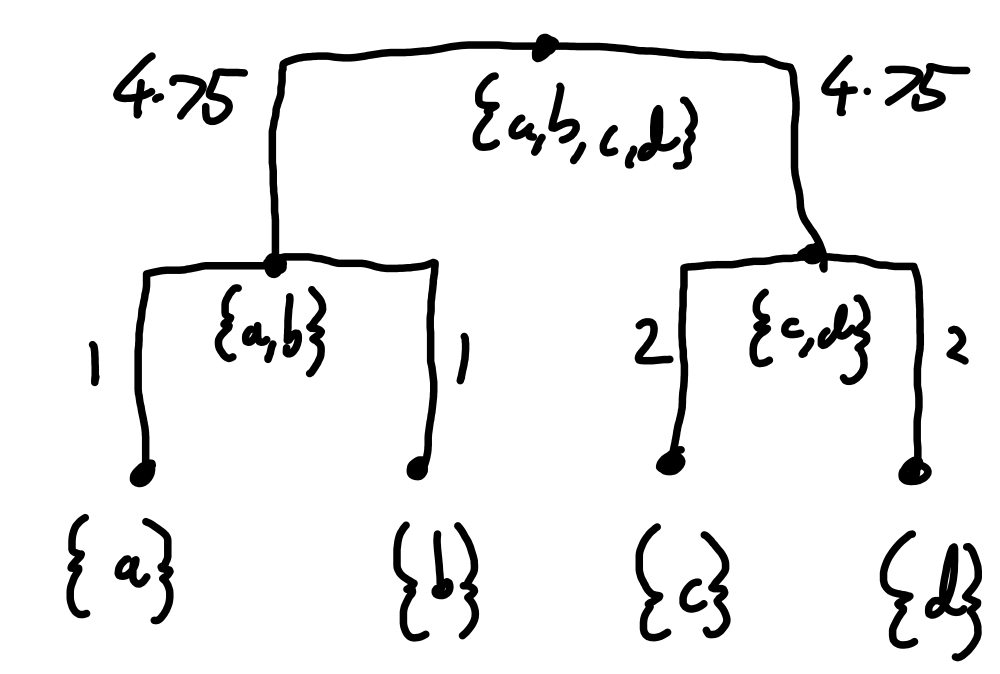
\includegraphics[scale=0.3]{upgma}

And the following intermediate distance matrices:


\begin{tabular}{c|c|c|c}
  &a,b&c&d\\
  \hline
  a,b&0&9&10\\
  \hline
  c& &0&4\\
  \hline
  d& & &0
\end{tabular}

\begin{tabular}{c|c|c}
  &a,b&c,d\\
  \hline
  a,b&0&9.5\\
  \hline
  c,d& &0\\
\end{tabular}

A trivial implementation of this algorithm has time complexity $O(n^3)$ and $O(n^2)$ space complexity, although an implementation exists that has $O(n^2)$ time complexity and $O(n^2)$ space complexity.

The UPGMA algorithm ensures that the resulting tree is ultrametric, meaning that every leaf is the same distance from the root. This means that we can interpret the resulting tree in an evolutionary context, where the distance between nodes and their ancesors are the time differences between the species.

The UPGMA algorithm can produce a tree for any distance matrix, unlike the additive phylogeny algorithm for example, but does not always produce the `best' trees. For example, if a matrix is additive, then we do not necessarily produce its corresponding simple tree, but an algorithm like neighbour-joining will.





\end{document}
